\documentclass[12pt]{article}
\title{ECE M16 Homework 4}
\usepackage{subcaption}
\author{Lawrence Liu}
\usepackage{graphicx}
\usepackage[english,shorthands=off]{babel}        % shorhands=off is required for babel french in combination with tikz karnaugh....
\usepackage[utf8x]{inputenc}
\usepackage[T1]{fontenc}
\usepackage{amsmath}
\usepackage{geometry}
\geometry{verbose,a4paper, tmargin=3.5cm,bmargin=3.5cm,lmargin=2.5cm,rmargin=2.5cm,headsep=1cm,footskip=1.5cm}
\usepackage{colortbl}
\usepackage[dvipsnames]{xcolor}
\usepackage{tikz -timing}
\usepackage{tikz}
\usepackage{listings}
\usetikzlibrary{karnaugh}

\definecolor{LogisimKMapColor0}{RGB}{128,0,0}
\definecolor{LogisimKMapColor1}{RGB}{230,25,75}
\definecolor{LogisimKMapColor2}{RGB}{250,190,190}
\definecolor{LogisimKMapColor3}{RGB}{170,110,40}
\definecolor{LogisimKMapColor4}{RGB}{245,130,48}
\definecolor{LogisimKMapColor5}{RGB}{255,215,180}
\definecolor{LogisimKMapColor6}{RGB}{128,128,0}
\definecolor{LogisimKMapColor7}{RGB}{255,255,25}
\definecolor{LogisimKMapColor8}{RGB}{210,245,60}
\definecolor{LogisimKMapColor9}{RGB}{0,0,128}
\definecolor{LogisimKMapColor10}{RGB}{145,30,180}
\definecolor{LogisimKMapColor11}{RGB}{60,180,175}
\definecolor{LogisimKMapColor12}{RGB}{0,130,203}
\definecolor{LogisimKMapColor13}{RGB}{230,190,255}
\definecolor{LogisimKMapColor14}{RGB}{170,255,195}
\definecolor{LogisimKMapColor15}{RGB}{240,50,230}


\definecolor{codegreen}{rgb}{0,0.6,0}
\definecolor{codegray}{rgb}{0.5,0.5,0.5}
\definecolor{codepurple}{rgb}{0.58,0,0.82}
\definecolor{backcolour}{rgb}{0.95,0.95,0.92}

\lstdefinestyle{mystyle}{
    backgroundcolor=\color{backcolour},   
    commentstyle=\color{codegreen},
    keywordstyle=\color{magenta},
    numberstyle=\tiny\color{codegray},
    stringstyle=\color{codepurple},
    basicstyle=\ttfamily\footnotesize,
    breakatwhitespace=false,         
    breaklines=true,                 
    captionpos=b,                    
    keepspaces=true,                 
    numbers=left,                    
    numbersep=5pt,                  
    showspaces=false,                
    showstringspaces=false,
    showtabs=false,                  
    tabsize=2
}

\lstset{style=mystyle}

\begin{document}
\maketitle
\section*{Problem 1}
\subsection*{(a)}
$$\boxed{220pS}$$
\subsection*{(b)}
$$\boxed{420pS}$$
\subsection*{(c)}
since the propagation delay is $420pS$, the clock cycle to satisfy the
setup time constraint is 
$$t_{cy}\geq t_{dCQ}+t_{dMax}+t_s$$
$$t_{cy}\geq 10pS+420pS+10pS$$
$$t_{cy}\geq \boxed{440pS}$$ 
\subsection*{(d)}
The hold time constraint with skew is 
$$t_h\leq t_{cCQ}+t_{cMin}-t_{k}$$
$$10pS \leq 10pS+220pS-t_k$$
$$t_k\leq220pS$$
However $t_k$ can be negative and the hold time constraint will still be satisfied, so the clock skew constraint is 
that clkd must be no later than 220pS after clk.
\subsection*{(e)}
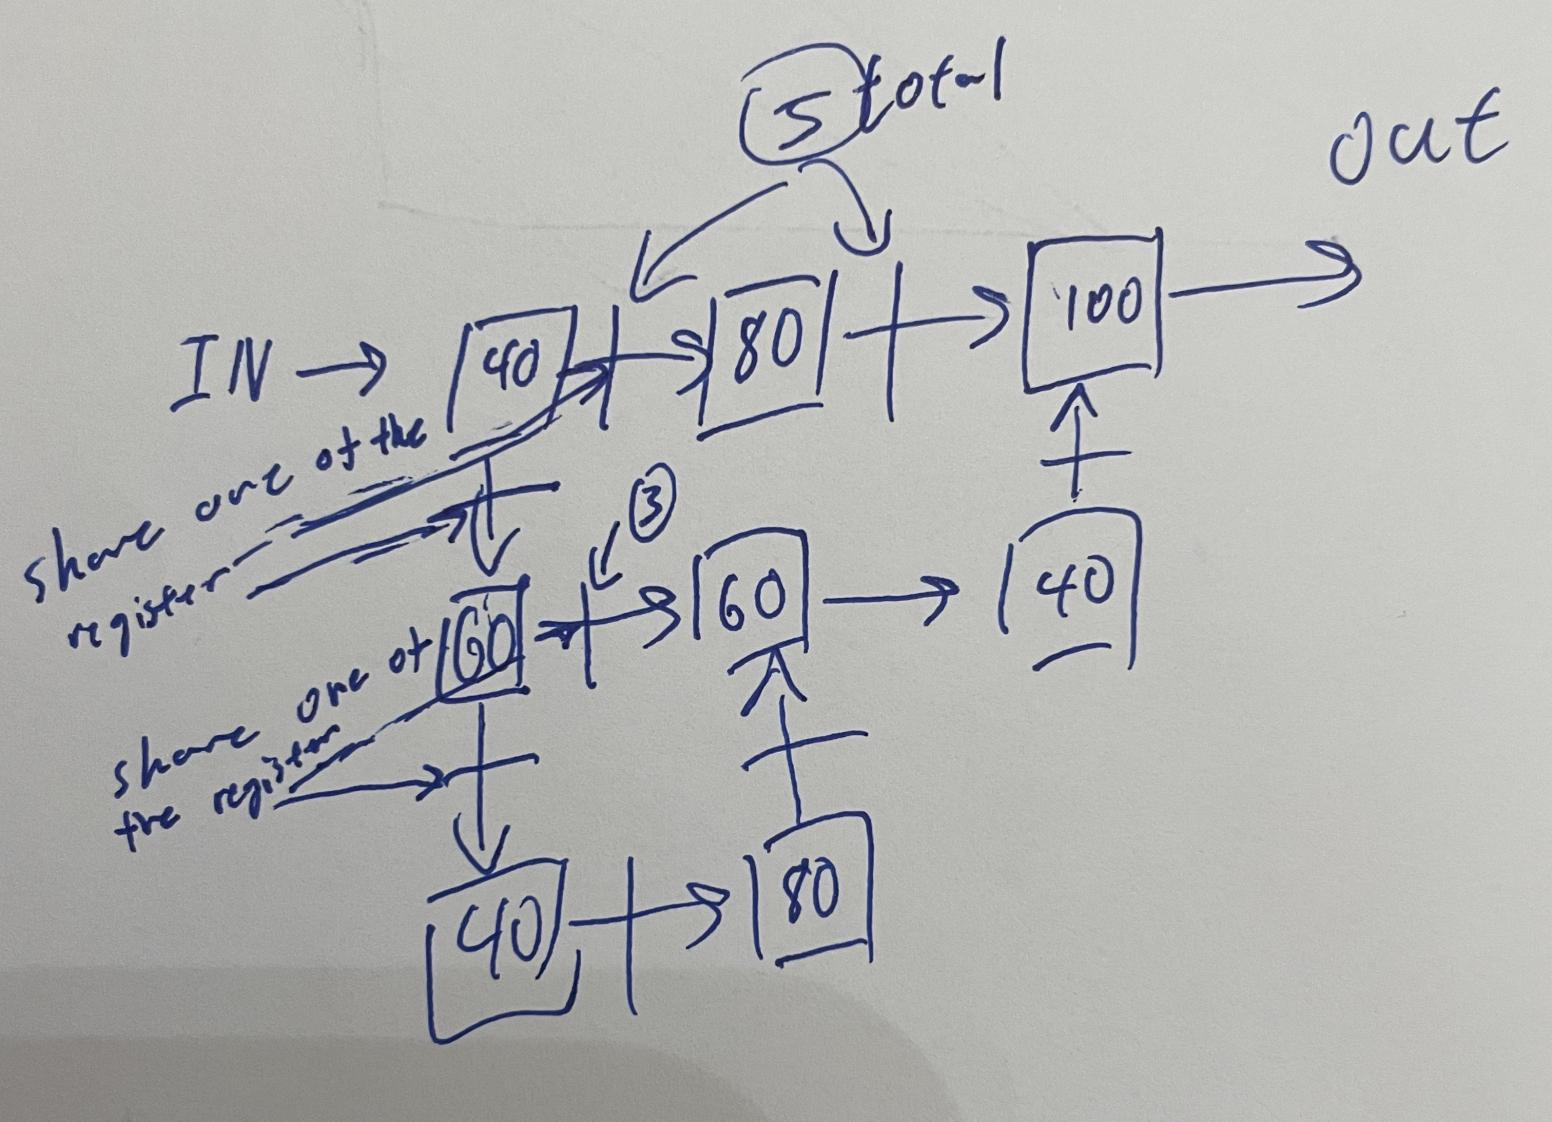
\includegraphics[scale=0.2]{Fig2.jpg}\\
placing registers as the vertical marks and placing multiple of them at the circled places to avoid timing problems, we can get it down to the bottleneck of the slowest moduel
so therefore the fastest clock cycle is 
$$t_{cy}\geq t_{dCQ}+t_{dMax}+t_s$$
$$t_{cy}\geq 10pS+100pS+10pS=\boxed{120pS}$$
This can be accomplished with 11 registers. I did not add a register after the 100pS block because it was connected straight to a register
\subsection*{(f)}
The signal would have to pass through 5 registers and given that the register overhead is 
$$t_{r}=t_{dCQ}+t_s=20pS$$
The latency is 
$$T=5(100pS+20pS)=\boxed{600pS}$$
\section*{Problem 2}
The flow table is \\
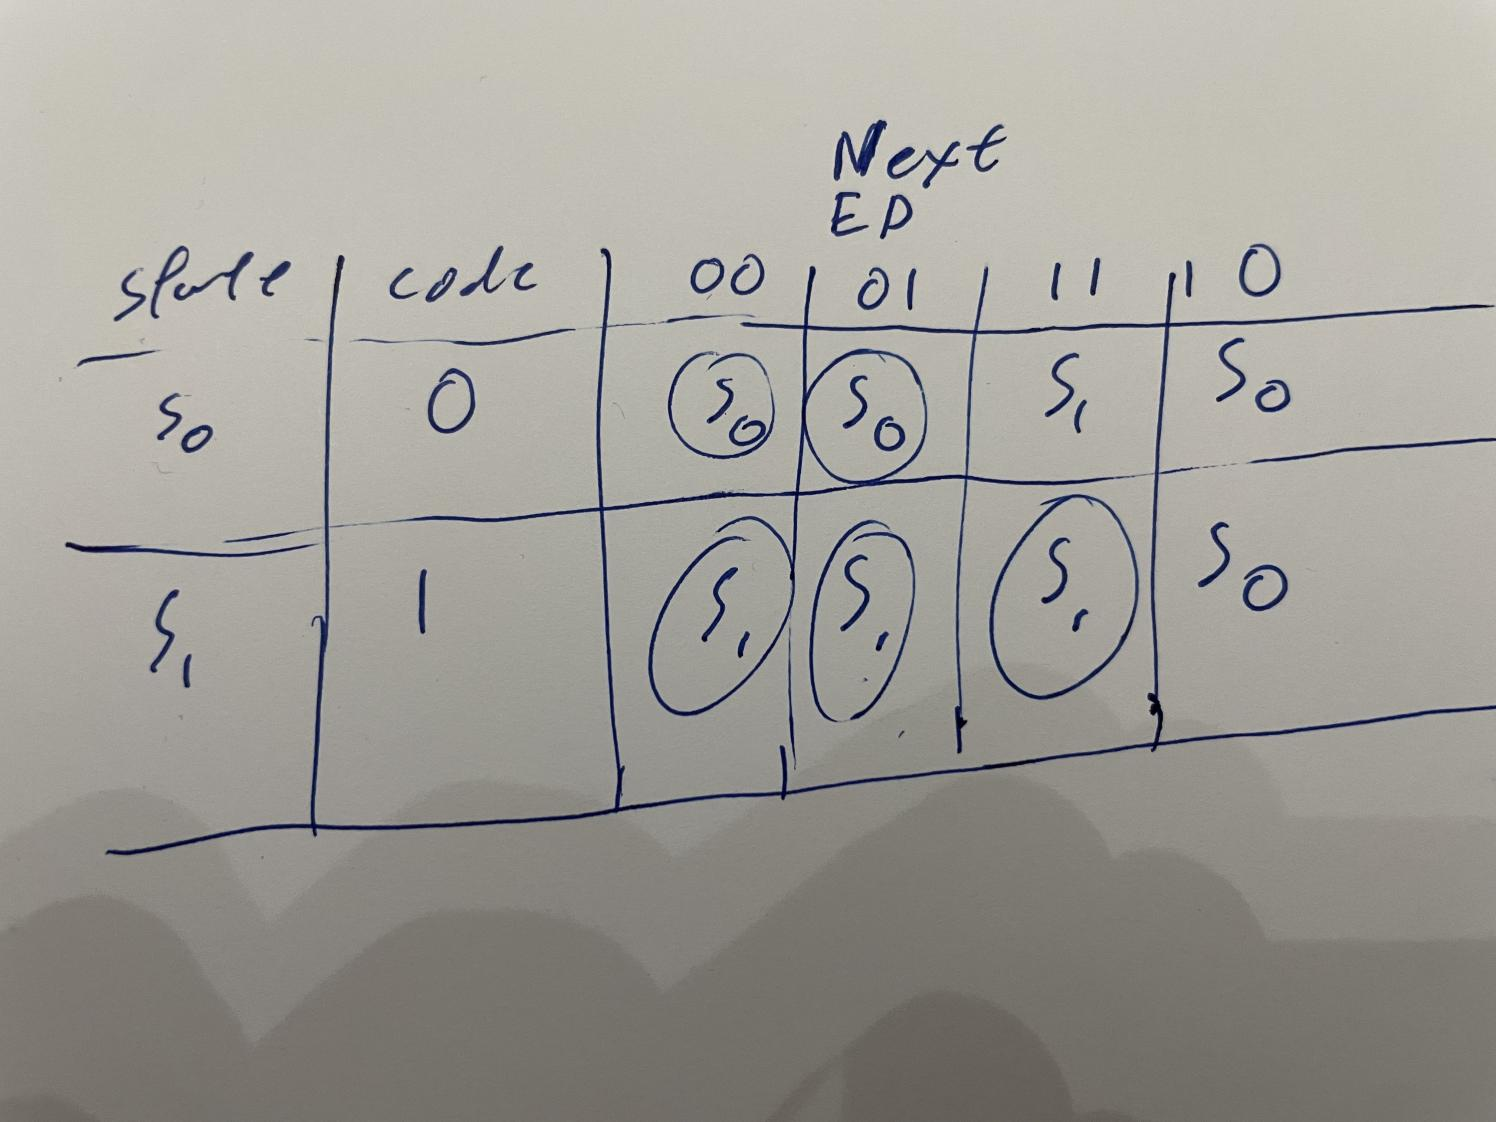
\includegraphics[scale=0.2]{Fig6.jpg}\\
Which results in the following kmap, \\
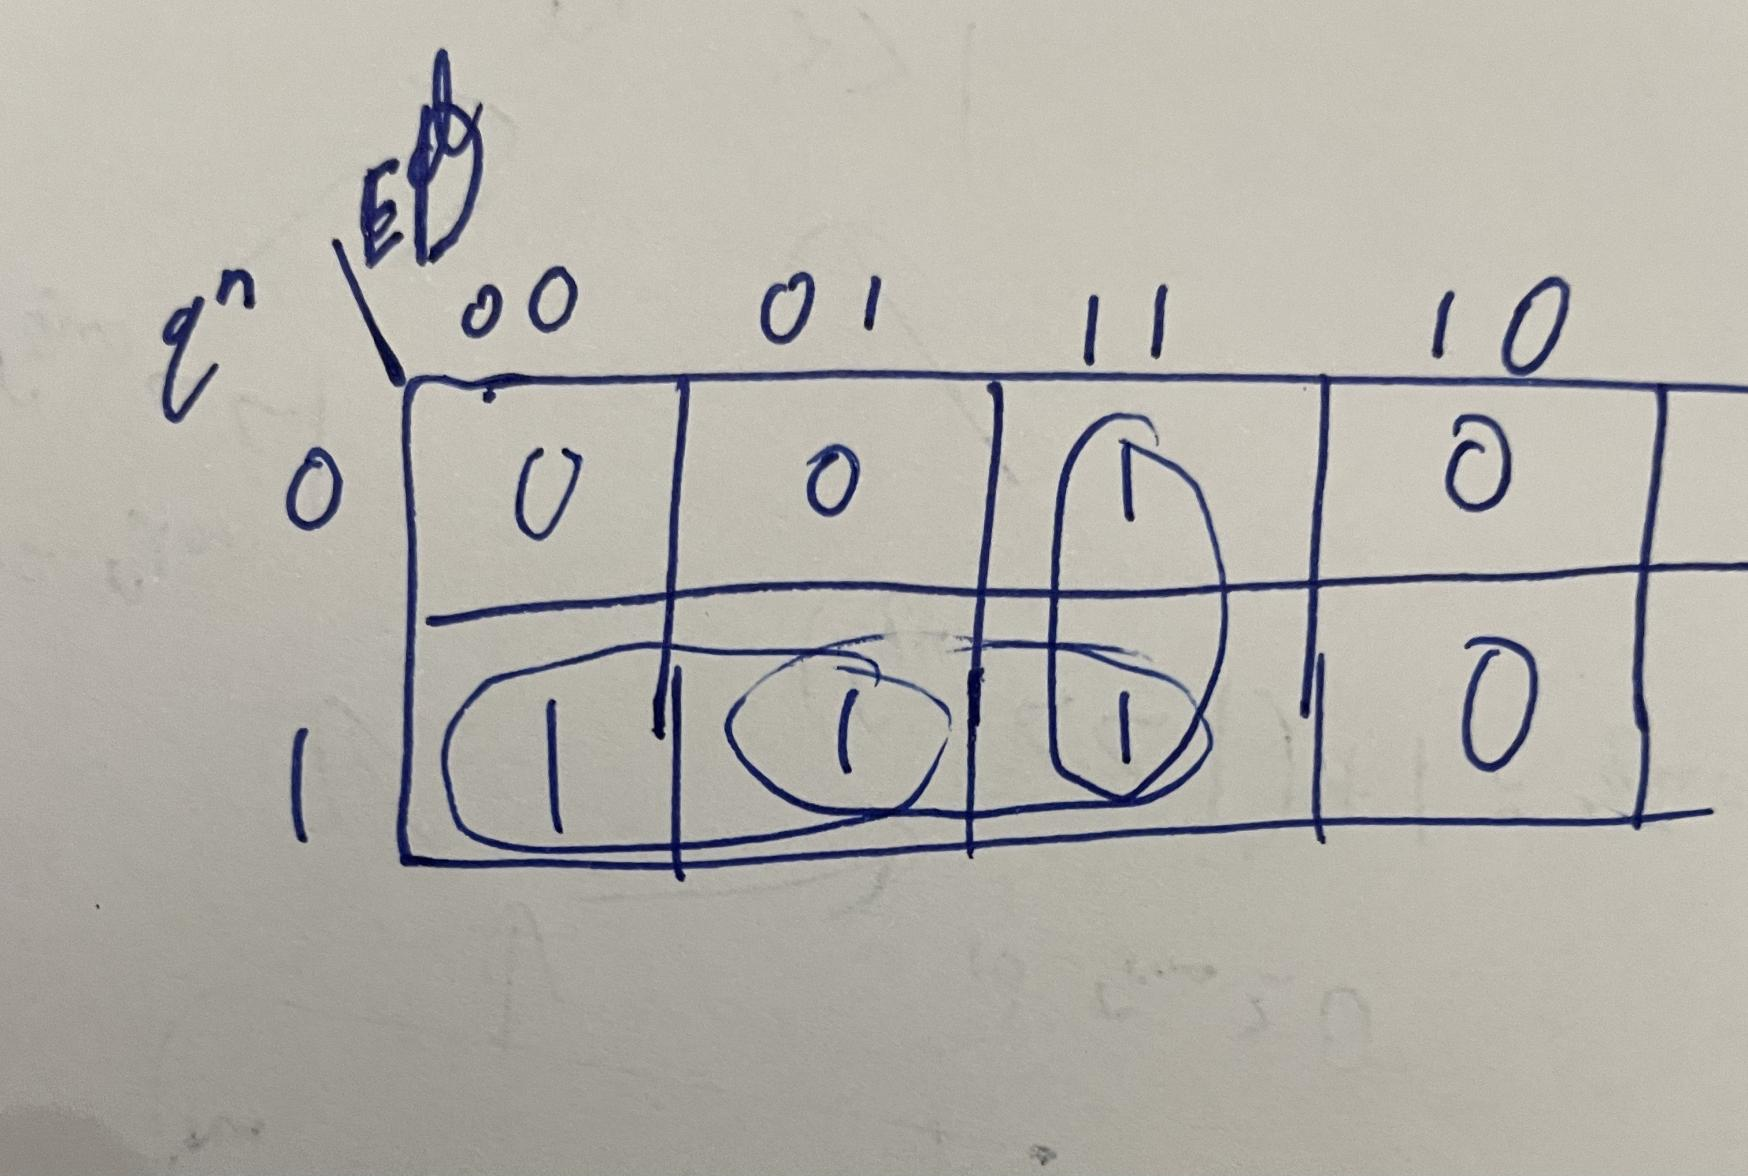
\includegraphics[scale=0.2]{Fig3.jpg}\\
And the following circuit\\
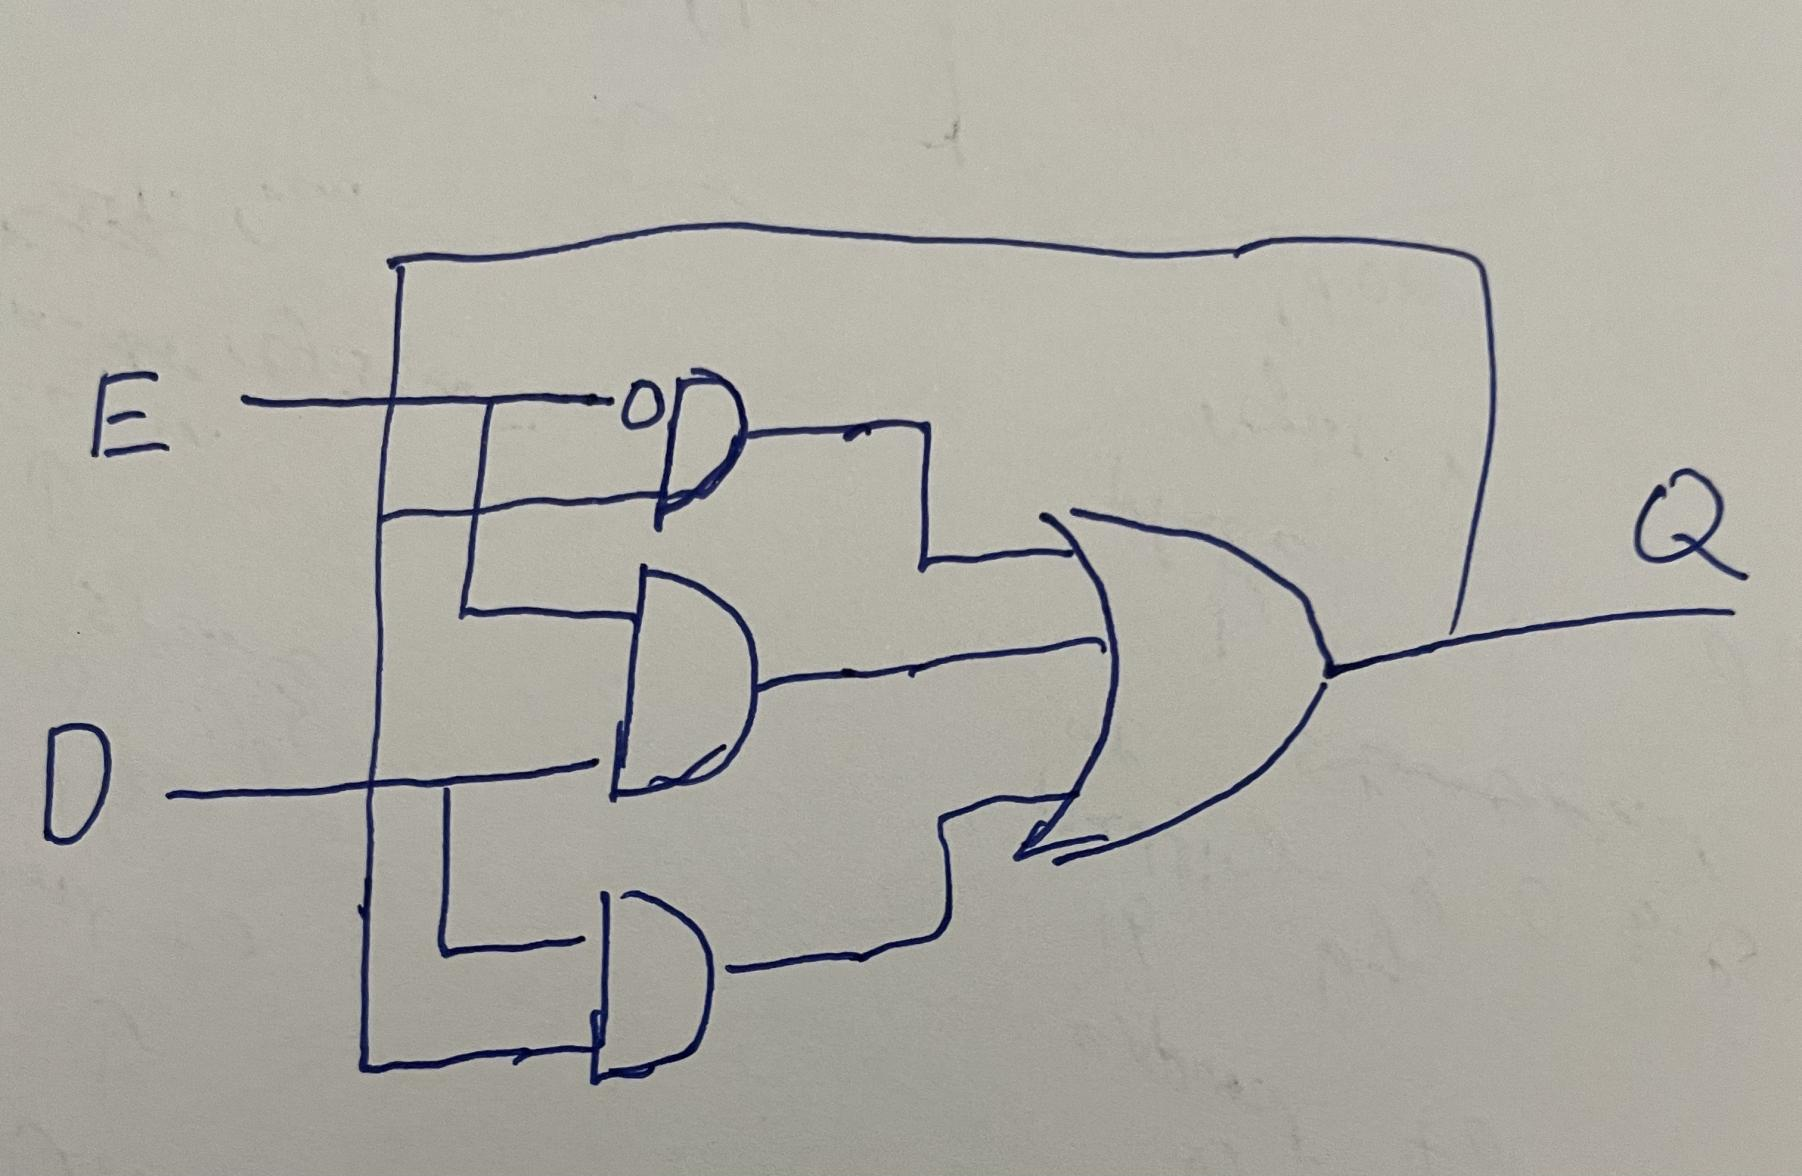
\includegraphics[scale=0.25]{Fig4.jpg}\\
Converting it to a flip flop involves just simply switching
E to the clock input C which results in the following circuit\\
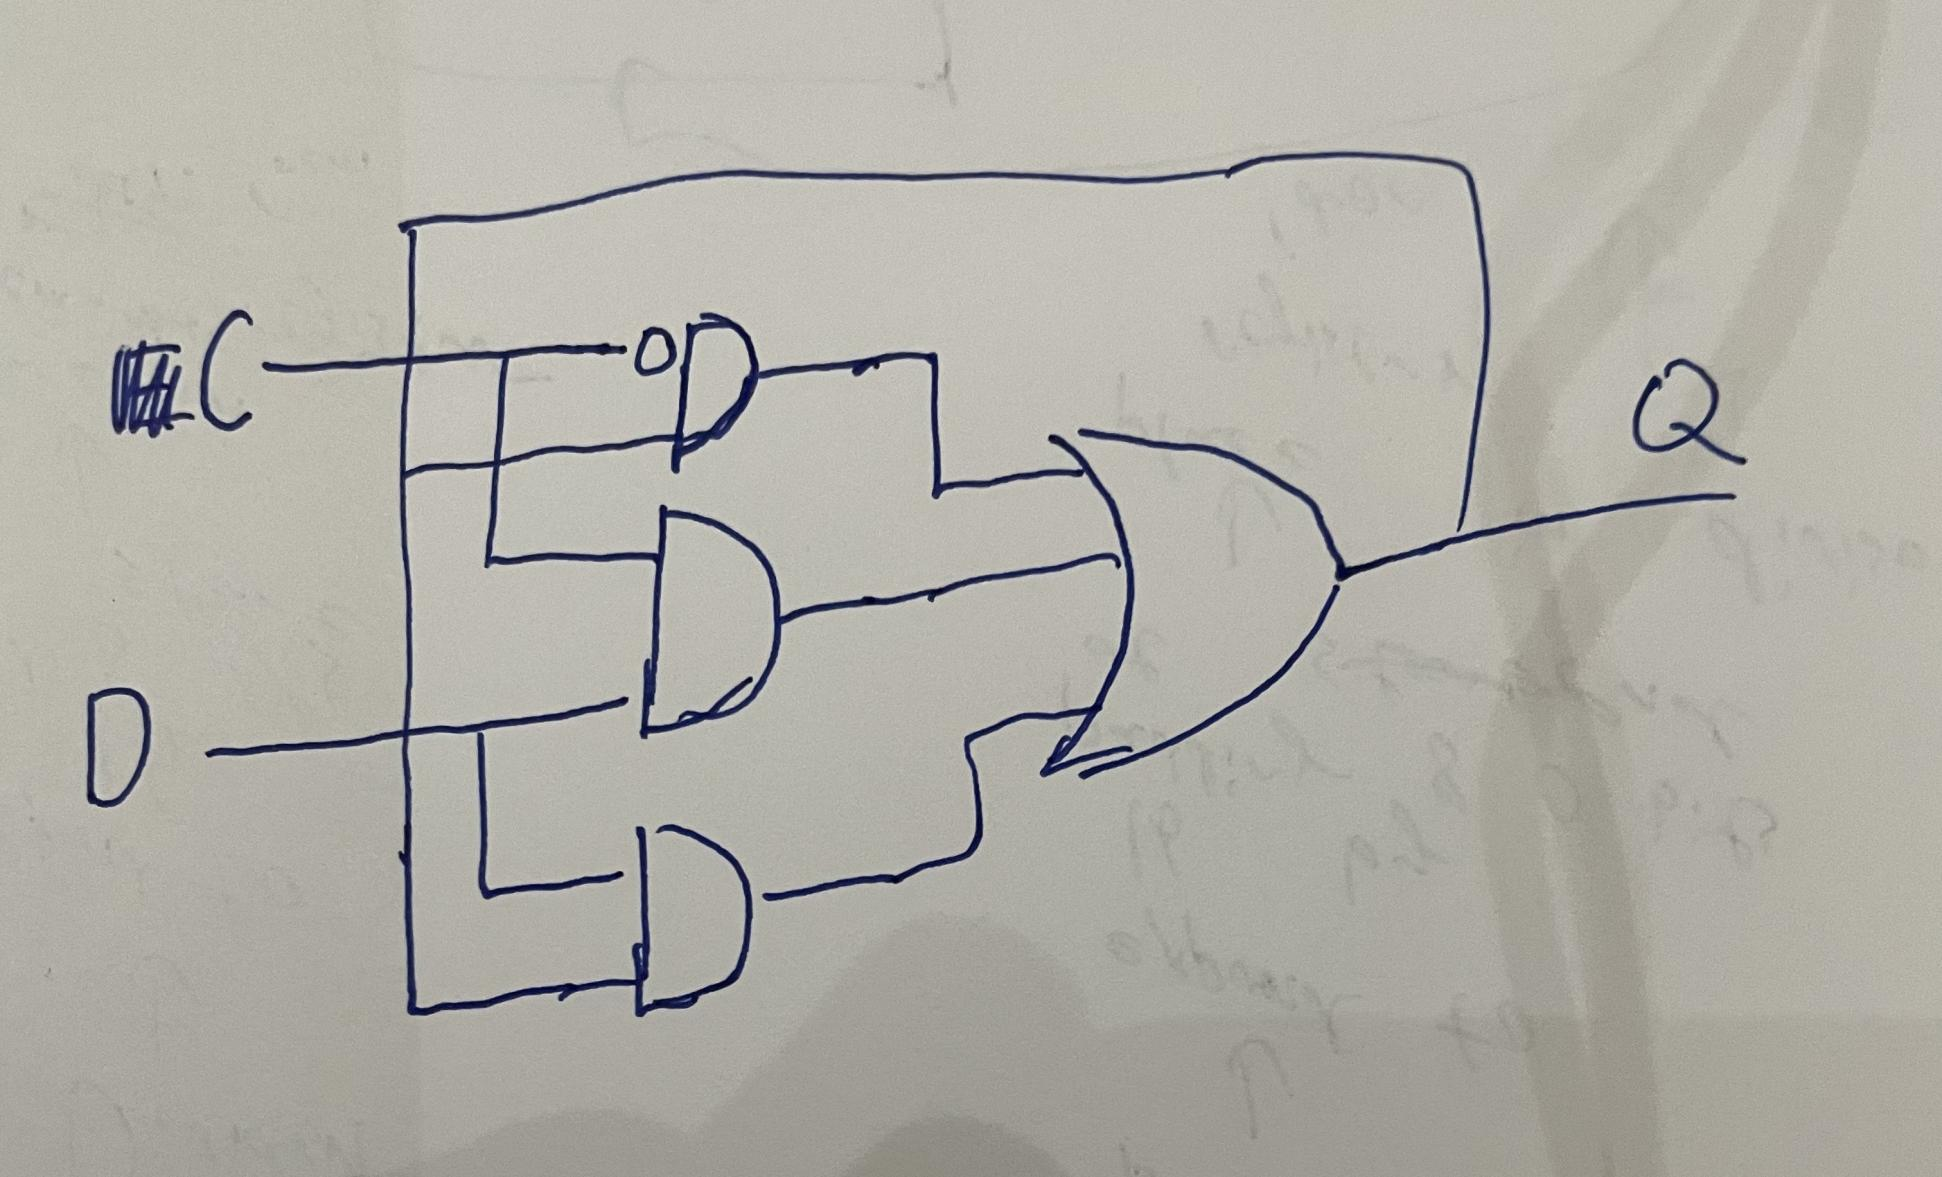
\includegraphics[scale=0.25]{Fig5.jpg}\\

Two of these are the same circuit as the one discussed in lecture.
\section*{Problem 3}
\subsection*{(a)}
$$Y_1=\overline{(\overline{y_1.c}).(\overline{y_3.d})}$$
$$Y_2=\overline{(\overline{y_1.c}).(\overline{y_3.y_2})}$$
$$Y_3=\overline{c.(\overline{y_1.c}).(\overline{y_3.d})}$$
\section*{(b)}
The state table is 
\begin{center}
    \begin{tabular}{|c|c|c|c|c|}
        Y1Y2Y3 & \multicolumn{4}{c}{cd} \\
        \hline
        & 00 & 01 & 11 & 10 \\
        \hline
        000 & 001& 001& 000& 000\\
\hline
001 & 001& 101& 101& 000\\
\hline
010 & 001& 001& 000& 000\\
\hline
011 & 011& 111& 111& 010\\
\hline
100 & 001& 001& 111& 111\\
\hline
101 & 001& 101& 111& 111\\
\hline
110 & 001& 001& 111& 111\\
\hline
111 & 011& 111& 111& 111\\
\hline
    \end{tabular}
\end{center}

or in terms of states
\begin{center}
    \begin{tabular}{|c|c|c|c|c|}
        Y1Y2Y3 & \multicolumn{4}{c}{cd} \\
        \hline
        & 00 & 01 & 11 & 10 \\
        \hline
        S0 & S1& S1& S0& S0\\
        \hline
        S1 & S1& S5& S5& S0\\
        \hline
        S2 & S1& S1& S0& S0\\
        \hline
        S3 & S3& S7& S7& S2\\
        \hline
        S4 & S1& S1& S7& S7\\
        \hline
        S5 & S1& S5& S7& S7\\
        \hline
        S6 & S1& S1& S7& S7\\
        \hline
        S7 & S3& S7& S7& S7\\
        \hline
    \end{tabular}
\end{center}

Keeping only the stable total states we get the following flow table
\begin{center}
    \begin{tabular}{|c|c|c|c|c|}
        Y1Y2Y3 & \multicolumn{4}{c}{cd} \\
        \hline
        & 00 & 01 & 11 & 10 \\
        \hline
        S0 & x& x& S0& S0\\
\hline
S1 & S1& x& x& x\\
\hline
S3 & S3& x& x& x\\
\hline
S5 & x& S5& x& x\\
\hline
S7 & x& S7& S7& S7\\
\hline
    \end{tabular}
\end{center}
This is the correct flow table for a d flip flop.
\section*{Problem 5}
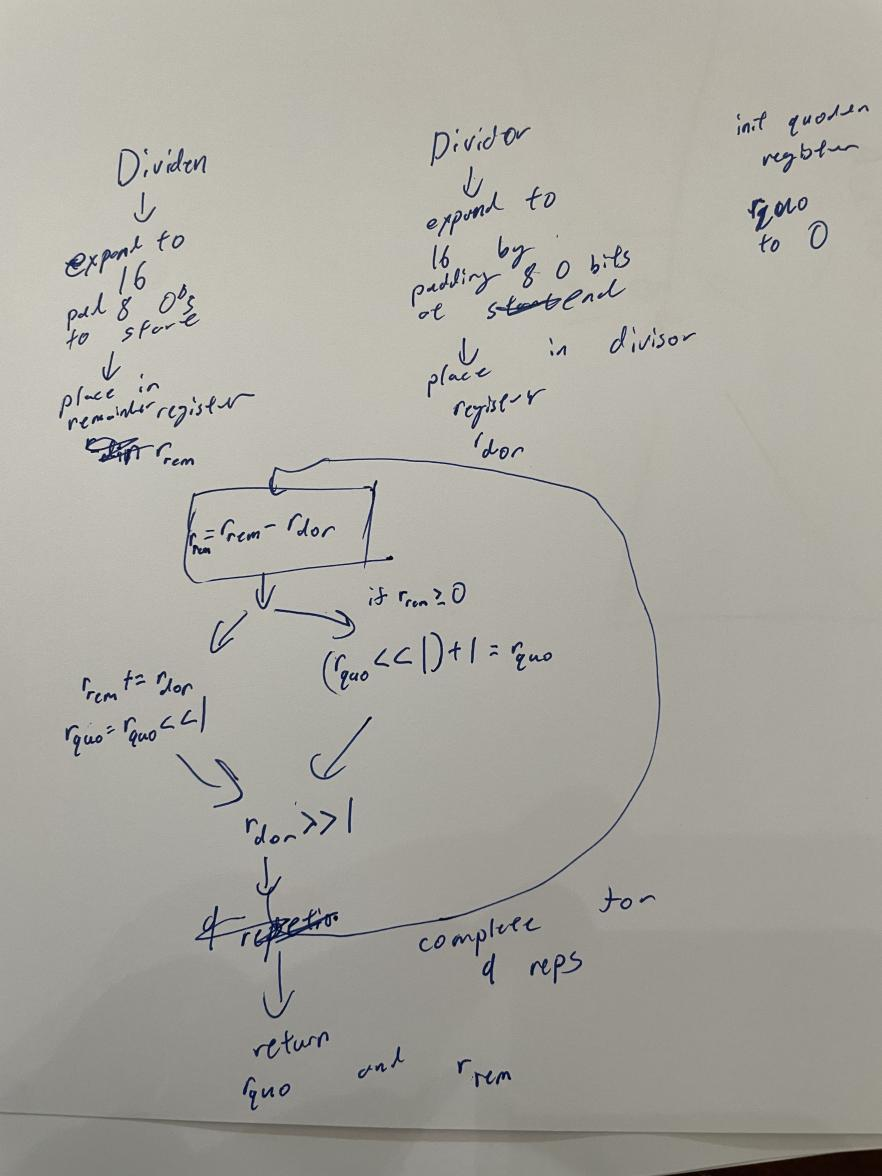
\includegraphics[scale=0.2]{Fig1.jpg}\\
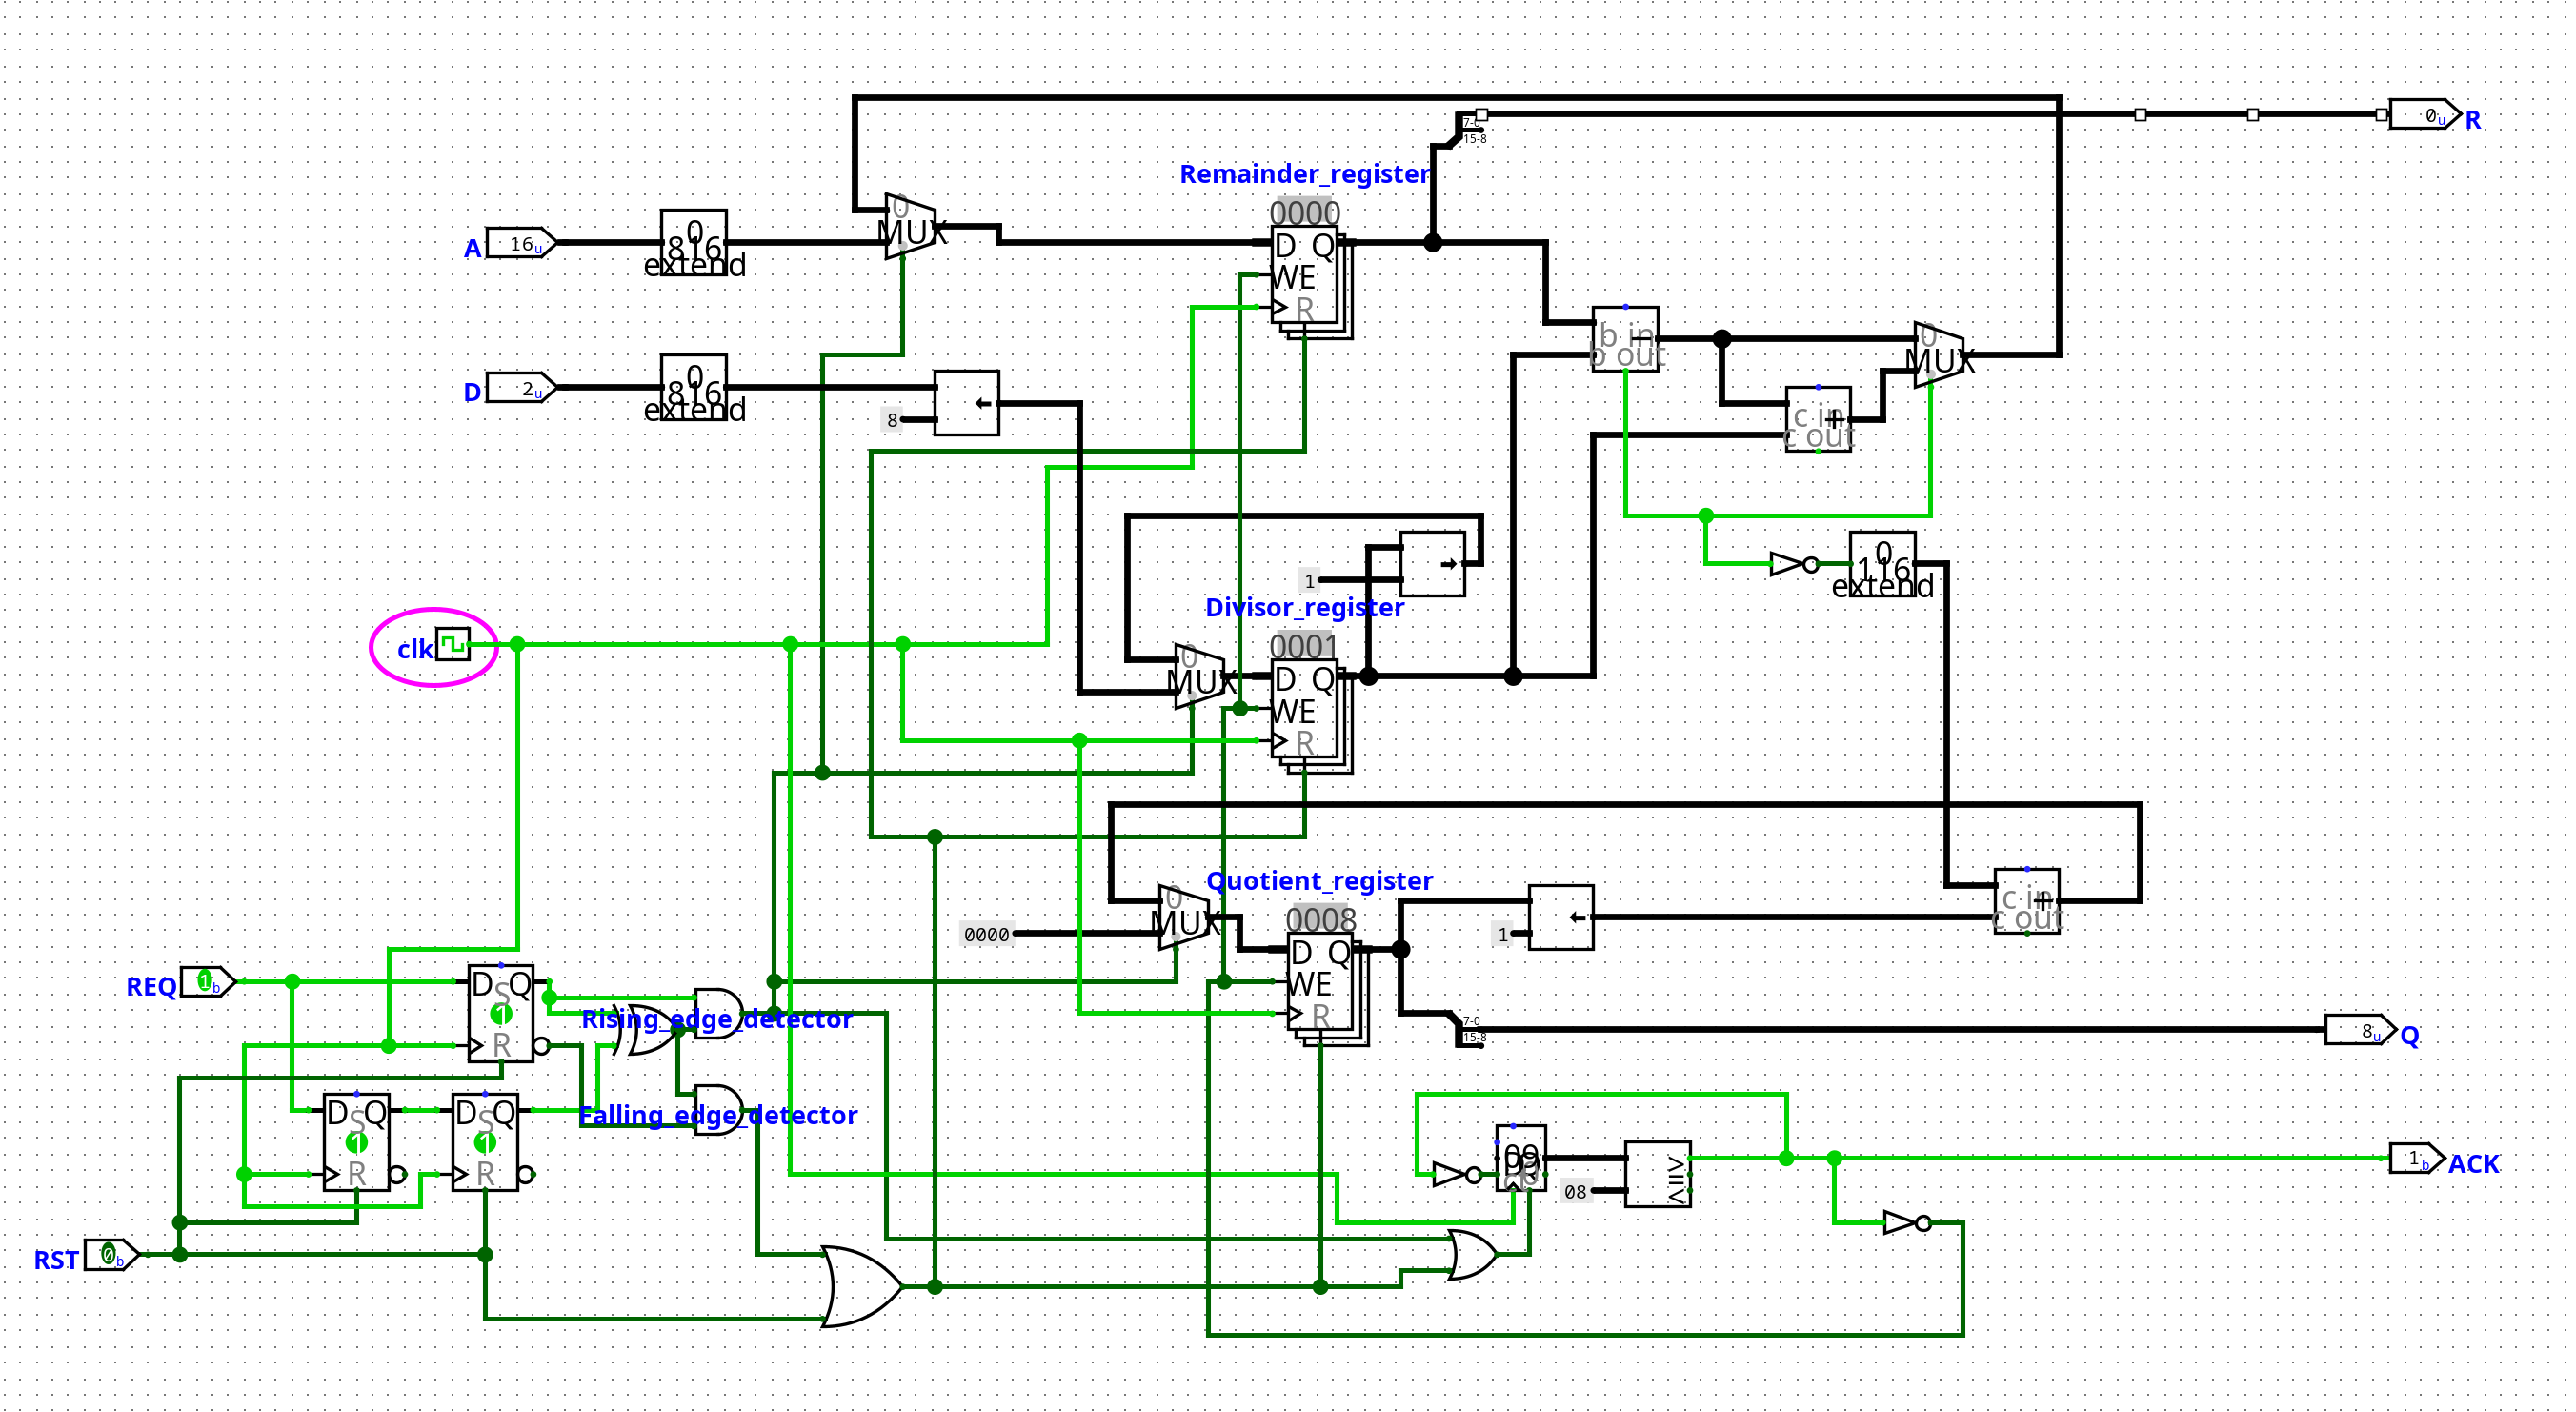
\includegraphics[scale=0.2]{Problem5.png}
\end{document}